\documentclass{article}
\usepackage[utf8]{inputenc}
\usepackage{graphicx}
\usepackage[spanish]{babel}
\usepackage{amssymb,amsmath,geometry}
\usepackage[hidelinks]{hyperref}
\usepackage{etoolbox} %titulo
\makeatletter %titulo
\patchcmd{\@maketitle}{\vskip 2em}{\vspace*{-3cm}}{}{} %titulo
\makeatother %titulo
\usepackage{vmargin}
\setpapersize{A4}
\setmargins{2.5cm}       % margen izquierdo
{1.5cm}                        % margen superior
{16.5cm}                      % anchura del texto
{23.42cm}                    % altura del texto
{10pt}                           % altura de los encabezados
{1cm}                           % espacio entre el texto y los encabezados
{0pt}                             % altura del pie de página
{2cm}                           % espacio entre el texto y el pie de página
\title{Cicloide}
\author{Aitor Moreno Rebollo y Andoni Latorre Galarraga}
\date{}
%comandos
\newcommand{\bb}[1]{\mathbb{#1}}
\newcommand{\R}{\bb{R}}
\begin{document}
\setlength{\parindent}{0cm}
\maketitle

\section{Descripción}
Si tomamos una circunferencia de radio $r$ y observamos la trayectoria que recorre el punto que comienza en el punto más bajo durante una vuelta completa, obtenemos una cicloide.
\begin{center}\begin{align*}
    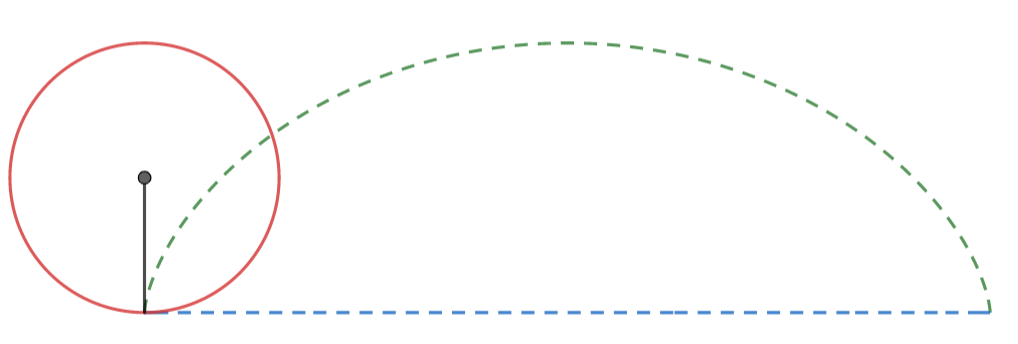
\includegraphics[scale=0.3]{figuras/cicloide descipcion 1.PNG}&
    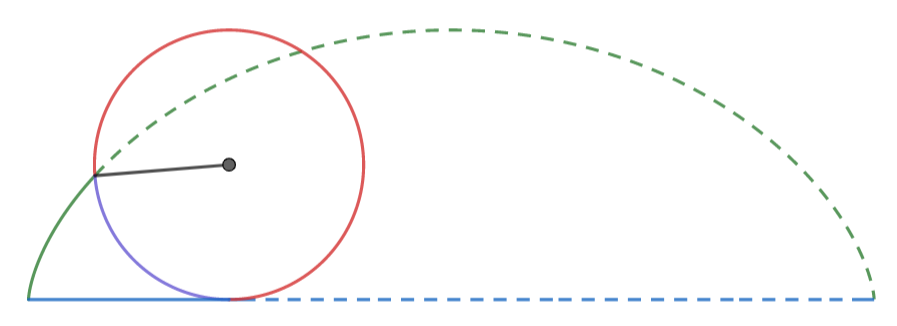
\includegraphics[scale=0.3]{figuras/cicloide descipcion 2.PNG}\\
    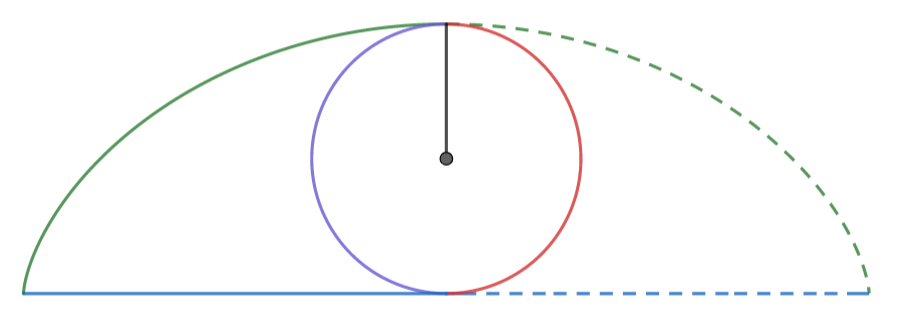
\includegraphics[scale=0.3]{figuras/cicloide descipcion 3.PNG}&
    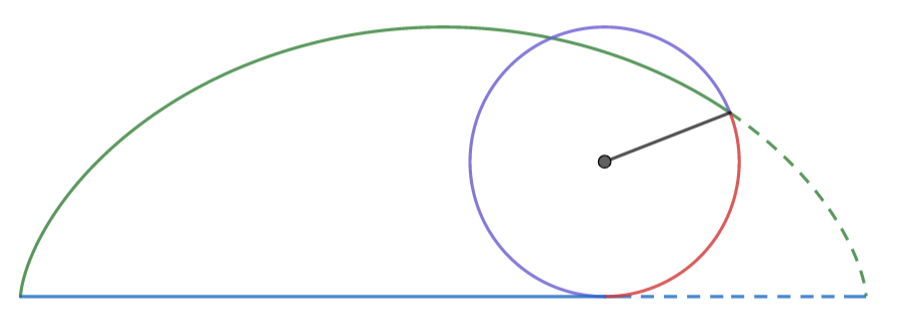
\includegraphics[scale=0.3]{figuras/cicloide descipcion 4.PNG}
\end{align*}
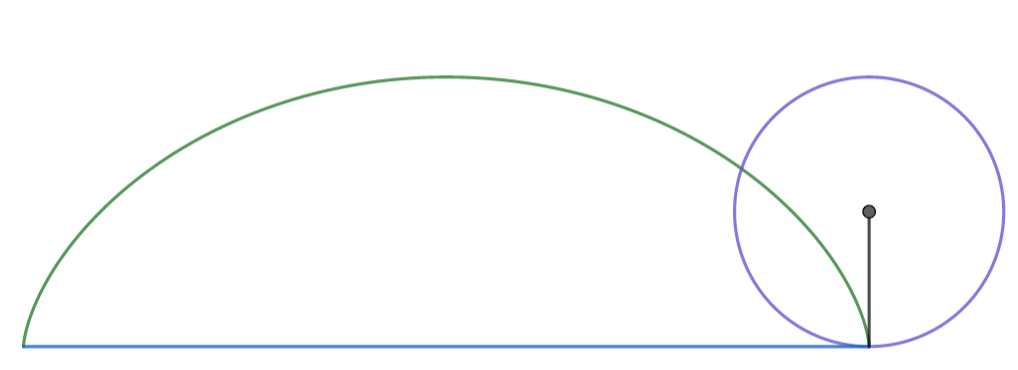
\includegraphics[scale=0.3]{figuras/cicloide descipcion 5.PNG}\\
\href{https://www.geogebra.org/calculator/ju6wnwpc}{Geogebra applet}
\end{center}
\section{Parametrización}
$$
\begin{array}{crcl}
\alpha : & (0,2\pi) & \longrightarrow & \bb{R}^2 \\
& t & \longmapsto     & (t-\sin(t),1-\cos(t))
\end{array}
$$
\section{Velocidad}
$$
\begin{array}{crcl}
\alpha' : & (0,2\pi) & \longrightarrow & \bb{R}^2 \\
& t & \longmapsto     & (1-\cos(t),\sin(t))
\end{array}
$$
\section{Diedro de Frenet}
Tenemos que $\begin{array}{crcl}
\alpha'' : & (0,2\pi) & \longrightarrow & \R^2 \\
& t & \longmapsto     & (\sin(t),\cos(t))
\end{array}$ y $\left\| \alpha'(t) \right\|=\sqrt{(1-\cos(t))^2+\sin^2(t)}$
\section{Longitud}
Para calcular la longitud de la cicloide evaluamos la siguiente integral
$$
\int_0^2\pi \left\| \alpha'(t) \right\| dt = \int_0^{2\pi} \sqrt{2-2\cos(t)} dt =\sqrt{2} \int_0^{2\pi} \sqrt{1-\cos(t)} dt
$$
$$
= \sqrt{2}\left[ -2 \sqrt{1-\cos(t)}\cot\left(\frac{t}{2}\right)\right]_0^{2\pi} = \sqrt{2}\sqrt{2}4=8
$$
\subsection{Parametrización por Longitud de arco}

\section{Curvatura}

\section{Curiosidades}
\subsection{Curva braquistócrona}
La palabra braquistócrona viene del griego \textit{braquistos} que significa el más corto y \textit{chronos} que significa tiempo, es decir, la curva que tiene el tiempo más corto. Si tenemos dos puntos $ P $, $ Q $ y queremos enncontrar la trayectoria que minimiza el tiempo de trayecto entre $ P $ y $ Q $. Obtenemos que dicha trayectoria es una cicloide.
\subsection{Curva tautócrona o isócrona}
Las palabras tautócrona e isócrona vienen de los prefijos griegos \textit{tauto/iso} que significan el mismo y de la palabra griega \textit{choronos} que significa tiempo, es decir, la curva tautócrona o isócrona es aquella en la que no importa el punto de partida, el tiempo requerido para llegar al punto más bajo es siempre el mismo. De nuevo, dicha curva es una cicloide.
\end{document}
